\documentclass[10pt, conference]{IEEEtran}
\hyphenation{op-tical net-works semi-conduc-tor}
\usepackage{graphicx}
\usepackage{fancyhdr}
\usepackage{url}
\usepackage{amsmath}
\usepackage{lipsum}
\usepackage{bookmark}
\usepackage{algorithm}
\usepackage{algorithmic}
\usepackage[normalem]{ulem}
\usepackage[usenames, dvipsnames]{color}
\usepackage[table,xcdraw]{xcolor}
\useunder{\uline}{\ul}{}
\def\code#1{\texttt{#1}}

\pagestyle{fancy}
\fancyhf{}
\lhead{\textsc{ELEN4020}}
\rhead{\textsc{Laboratory Exercise No 2}}
\rfoot{Page \thepage\ }


\begin{document}
\begin{titlepage}
\newcommand{\HRule}{\rule{\linewidth}{0.5mm}} % Defines a new command for the horizontal lines, change thickness here

\center % Center everything on the page
 
%----------------------------------------------------------------------------------------
%	HEADING SECTIONS
%----------------------------------------------------------------------------------------

\textsc{\LARGE University of Witwatersrand}\\[1.5cm] % Name of your university/college
%----------------------------------------------------------------------------------------
%	LOGO SECTION
%----------------------------------------------------------------------------------------


\includegraphics[scale=0.25]{Wits.png}% Include a department/university logo - this will require the graphicx package
 
 
%----------------------------------------------------------------------------------------
\textsc{\Large ELEN4020}\\[0.5cm] % Major heading such as course name
\textsc{\large Data Intensive Computing In Data Science}\\[0.5cm] % Minor heading such as course title



%----------------------------------------------------------------------------------------
%	TITLE SECTION
%----------------------------------------------------------------------------------------

\HRule \\[0.4cm]
{ \huge \bfseries Laboratory Exercise 2}\\[0.4cm] % Title of your document
\HRule \\[1.5cm]
 
%----------------------------------------------------------------------------------------
%	AUTHOR SECTION
%----------------------------------------------------------------------------------------

\begin{minipage}{0.4\textwidth}
\begin{flushleft} \large
	\emph{Authors:}\\
	\textsc{Kishan Narotam - 717 931\\Jesal Chana - 603 177} 
\end{flushleft}
\end{minipage}
~
\begin{minipage}{0.4\textwidth}
\begin{flushright} \large
	\emph{Authors:} \\
	\textsc{Syed Hussain - 600 524\\Yusuf Ally - 604 973} 
\end{flushright}
\end{minipage}\\[2cm]

%----------------------------------------------------------------------------------------
%	DATE SECTION
%----------------------------------------------------------------------------------------

{\large 9\textsuperscript{th} March 2018}\\[2cm] % Date, change the \today to a set date if you want to be precise

%-------------------------------------------------------------------------------------

\vfill % Fill the rest of the page with whitespace

\end{titlepage}
%----------------------------------------------------------------------------------------


%----------------------------------------------------------------------------------------
%	MAIN BODY OF REPORT
%----------------------------------------------------------------------------------------

\section{Problem Description}
\label{Problem Description}
A square matrix, defined as $A[N_0][N_1]$, must be created with various dimensions, where $N_0 = N_1 = 128, 1024,8192$. The matrix could be an integer which is 4 bytes or a short floating point which too is 4 bytes. The elements of the matrix must be generated using the formula presented in equation~\ref{eqn1}:
\begin{equation}
\label{eqn1}
\begin{split}
A\langle i, j\rangle & = i *N_j + j
\end{split}
\end{equation}

The transpose of these matrices must be computed without wasting memory by creating a copy of the original matrix, but rather modify the original matrix to become the transposed matrix. Since the size of the matrix is so large, PThread and OpenMP programming must be performed on the matrix. The number of threads that must be used are $4,8,16,128$ for each value of $N_0$. The time taken to perform the transposition of each matrix must be recorded.

\section{Background}
\label{Background}

\subsection{PThread}
\label{PThread}
A thread is a set of instructions that are independent and scheduled to run by the operating system. A POSIX Thread (PThread) however is defined as a standardized programming interface for UNIX systems, i.e. an execution model independent of any programming language. It could also be defined as a set of \emph{C} language programming types, functions, procedures and constants that are implemented with the library header file, \code{pthread.h}~\cite{PThread}.

PThreads are also regarded as low-level application programming interface (API) when managing threads. It allows the user to have as refined control as possible over the threads as well as multiple exclusion objects~\cite{StackOverflow}. Since the Pthreads are such low level, it is fairly limited to the language used.

\subsection{OpenMP}
\label{OpenMP}
Open Multi-Processing (OpenMP) is an API that is used explicitly to direct multi-threading and shared memory parallelism. It is comprised of three primary API components:

\begin{itemize}
\item Compiler Directives
\item Runtime Library Routines
\item Environment Variables\cite{OpenMP}.
\end{itemize}

OpenMP is a much higher level API, and portable allowing the user to utilize this API in different languages such as C, C++ and Fortran. It is more easily scaled than PThreads as it has the ability to divide the work across multiple threads with ease~\cite{StackOverflow, OpenMP}.

For this type of problem, the program that utilizes OpenMP should reveal faster times than the program that utilizes PThreads.

\subsection{Amdahl's Law}
\label{Amdahl's Law}
Amdahl's Law is a key concept that is used to understand in parallel computing. It is used to predict the maximum speedup in latency for a program processing using multiple processors~\cite{Amdahl}.

In parallel computing, the law states that if $P$ is the program that can be made parallel, i.e. proportion of execution time, and given that $1-P$ is the remaining proportion, i.e. the proportion that is still serial, the maximum speedup in latency using $N$ number of processors can be defined as equation~\ref{eqn2}.

\begin{equation}
\label{eqn2}
\begin{split}
S_{latency} = \frac{1}{(1-P)+\frac{P}{N}}
\end{split}
\end{equation}

The speedup is limited by the total time needed for the serial proportion of the program. For example is a program need 10 hours using a single processor, and 9 hours can be parallelized, and 1 cannot, the maximum speedup is limited to $10\times$ using equation~\ref{eqn2}~\cite{Amdahl}.

\section{Function Description}
\label{Function Description}

\subsection{Transpose method}
The input matrix \code{array} is transposed by swapping element $A[i,j]$ with $A[j,i]$. Note only elements in the upper triangle of the array are transposed. For a square matrix of width $N$, the number of upper triangle elements $\Delta$ is given by 

\begin{equation}
\Delta = \frac{N^2 - N}{2}
\end{equation}
A second array, \code{utArray}, is populated with only the indices of upper triangle elements of \code{array}. In this way, only $\Delta$ elements need to be traversed in order to do the transpose. \code{utArray} is therefore a 1D array of size $\Delta$. As \code{utArray} is traversed, it's corresponding 2D coordinate in \code{array} is obtained using
\begin{equation}
row = i~/~N\\
\end{equation}
and \begin{equation}
column = i~\%~N
\end{equation}
Where $i$ is the index of a particular element. For example a 4x4 matrix given as\\

\centering
 
$Array = \left[\begin{array}{cccc}
0 & \colorbox{Goldenrod}{1} & \colorbox{Goldenrod}{2} & \colorbox{Goldenrod}{3}	\\
4 & 5 & \colorbox{Goldenrod}{6} & \colorbox{Goldenrod}{7}	\\
8 & 9 & 10 & \colorbox{Goldenrod}{11}	\\
12 & 13 & 14 & 15
\end{array}\right]$
\flushleft
will produce an upper triangle matrix\newline\\
\centering
$ utArray = \left[\begin{array}{cccccc}
\colorbox{Goldenrod}{1} & \colorbox{Goldenrod}{2} & \colorbox{Goldenrod}{3} & \colorbox{Goldenrod}{6}& \colorbox{Goldenrod}{7}& \colorbox{Goldenrod}{11}
\end{array}\right]$
\flushleft
Example : choose element '6' in \code{utArray}; $i = 6$.\\
\centering
$\rightarrow row = i~/~N = 6~/~4 = 1$ (integer division)\\
$\rightarrow column = i~\%~N = 6~\%~4 = 2$ (modulo division)\\
\flushleft
So at coordinate (1,2) in \code{array}, the value is 6 as expected. This is then swapped with the element at (2,1) in \code{array} - which is 9. This process is repeated for every element in \code{utArray}.

\subsection{Multithreading approach}
For optimal performance, it is desirable to have the workload divided equally between all threads. In this case it means having each thread to the same amount of transposes. For this, we calculate $\alpha$, which is the number of elements in \code{utArray} to traverse per thread.
\begin{equation}
\alpha = \frac{\Delta}{Threads}
\end{equation}

So for our previous 4x4 matrix, using 2 threads~($Threads = 2$),\newline\newline
\centering
$\alpha = \frac{\Delta}{Threads} = \frac{6}{2} = 3$
\flushleft
This means thread 0 transposes the first three elements in \code{utArray}, and thread 1 transposes the next three elements.

\centering
$Array = \left[\begin{array}{cccc}
0 & \colorbox{Goldenrod}{1} & \colorbox{Goldenrod}{2} & \colorbox{Goldenrod}{3}	\\
4 & 5 & \colorbox{green}{6} & \colorbox{green}{7}	\\
8 & 9 & 10 & \colorbox{green}{11}	\\
12 & 13 & 14 & 15
\end{array}\right]$
\flushleft
then\\
\centering
$ utArray = \left[\begin{array}{cccccc}
\colorbox{Goldenrod}{1} & \colorbox{Goldenrod}{2} & \colorbox{Goldenrod}{3} & \colorbox{green}{6}& \colorbox{green}{7}& \colorbox{green}{11}
\end{array}\right]$\\
\flushleft
Here the yellow highlighted elements are processed by thread 0, and the green highlighted elements are processed by thread 1.

\subsection{\code{transposeBlock}}
This is the function that executes the transpose of each upper triangle element. It takes as arguments the starting point index for each thread, \code{sp}, and the number of elements per thread, \code{alpha}. It then takes the index value from \code{utArray} (using \code{utArr\_ptr}) and gets the corresponding row (\code{r}) and column (\code{c}) values in \code{Array}. Using this row and column value, the element is then transposed.


\section{Pseudo Code}
\label{Pseudo Code}

The pseudo code for the entire program is seen in Appendix~\ref{Pseudo Appendix}. Although written in one file, the pseudo code is done in such a way that each method/function is split into their own algorithms. Algorithm~\ref{Struct} in Appendix~\ref{Pseudo Appendix} is the defined \code{struct} for the thread. Algorithm~\ref{transposeBlock} in Appendix~\ref{Pseudo Appendix} is the function to transpose the matrix. Algorithms~\ref{main},~\ref{Normal Transposition} and \ref{PThread Transposition} are all within the \code{main} class. Algorithms~\ref{Normal Transposition} and \ref{PThread Transposition} were commented out during testing so that each individual time could be recorded for the results presented in Table~\ref{Results}.

\section{Final Code and Output}
\label{Final Code and Output}

The final programs were coded in \emph{C} on an \emph{Ubuntu} system and compiled using a custom makefile. Table~\ref{Results} shows the times recorded for each of the square matrices defined in Section~\ref{Problem Description}. Each matrix was tested three times and the average time taken to transpose the matrix using no threading, PThread and OpenMP was recorded. The time is recorded in milliseconds and is tested on a machine with the following specifications.

\subsection{Testing Machine}
\label{Testing Machine}
An ASUS N550JV high performance laptop was used for testing. The machine has an \emph{Intel(R) Core(TM) i7-4700HQ CPU} with $12GB$ of RAM installed with a 64-bit operating system installed. The operating system installed is \emph{Windows 10 Pro} however for testing, a virtual machine was installed with the \emph{Ubuntu 16.04.3} 64-bit installed. $5GB$ of the total RAM is dedicated to the virtual machine. The following code was run in the terminal to determine the total number of threads in a shared memory space:

\code{cat /proc/sys/kernel/threads-max}

The output of this command was $38255$.

\begin{table}[h!]
\centering
\caption{Table showing time taken to transpose the matrices using no threading, PThread and OpenMP}
\label{Results}
\begin{tabular}{|r|c|c|c|}
\hline
\multicolumn{1}{|l|}{{\ul \textbf{N0 = N1}}} & {\ul \textbf{128}} & {\ul \textbf{1024}} & {\ul \textbf{8192}} \\ \hline
\multicolumn{4}{|c|}{\cellcolor[HTML]{C0C0C0}{\ul \textbf{No threading}}}                                     \\ \hline
\multicolumn{1}{|c|}{}                       & 0.036              & 7.004               & 1367.784            \\ \hline
\multicolumn{4}{|c|}{\cellcolor[HTML]{C0C0C0}{\ul \textbf{PThread}}}                                          \\ \hline
\textbf{4}                                   & 0.086              & 0.109333            & 0.125333            \\ \hline
\textbf{8}                                   & 0.191              & 0.324667            & 0.204333            \\ \hline
\textbf{16}                                  & 0.292              & 0.366333            & 0.392667            \\ \hline
\textbf{64}                                  & 1.063333           & 12.287              & 170.9217            \\ \hline
\textbf{128}                                 & 2.269667           & 16.59567            & 712.026             \\ \hline
\multicolumn{4}{|c|}{\cellcolor[HTML]{C0C0C0}{\ul \textbf{OpenMP}}}                                           \\ \hline
\textbf{4}                                   &                    &                     &                     \\ \hline
\textbf{8}                                   &                    &                     &                     \\ \hline
\textbf{16}                                  &                    &                     &                     \\ \hline
\textbf{64}                                  &                    &                     &                     \\ \hline
\textbf{128}                                 &                    &                     &                     \\ \hline
\end{tabular}
\end{table}

\section{Different Methods}
\label{Different Methods}

\subsection{Splitting the Matrix}
\label{Splitting the Matrix}
Since parallel computing can be used, another method that can be used to transpose a matrix would be to split the matrix into smaller matrices and giving each thread a smaller matrix to transpose. Figure~\ref{Splitting} gives an example an $8\times8$ matrix that is split into four smaller matrices and 4 threads would be applied to this. Each thread handles a smaller $4\times4$ matrix and processes the matrix and calculates the transpose.

Although an efficient method, this would be poor on the memory. The reason for this is that an index would have to be created in order to track which elements have already been transposed. This is a trade off of this method, where efficiency is improved however memory is wasted.

\begin{figure}[h!]
\renewcommand{\thefigure}{\arabic{figure}}
\centering
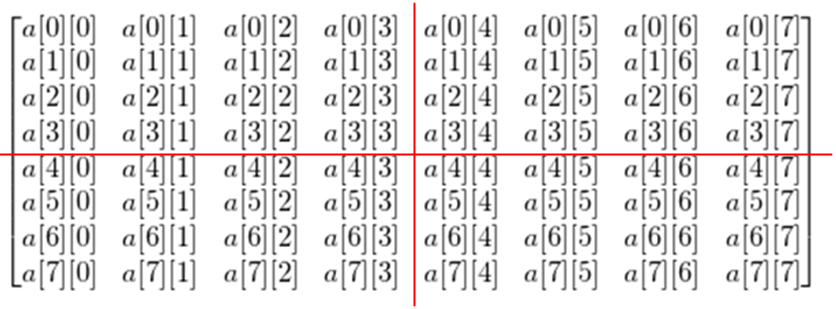
\includegraphics[scale=0.35]{Splitting.png}
\caption{An $8\times8$ matrix that is split into smaller $4\times4$ matrices}
\label{Splitting}
\end{figure}

\section{Conclusion}
\label{Conclusion}
The conclusion goes here.


\begin{thebibliography}{}

\bibitem{PThread}
Barney, B; Livermore, L; \emph{POSIX Threads Programming}; \url{https://computing.llnl.gov/tutorials/pthreads/}; Last Accessed: 01/03/2018

\bibitem{StackOverflow}
Ball, M; \emph{c - Pthreads vs. OpenMP - Stack Overflow}; \url{https://stackoverflow.com/questions/3949901/pthreads-vs-openmp}; Last Accessed: 01/03/2018

\bibitem{OpenMP}
Barney, B; Livermore, L; \emph{OpenMP}; \url{https://computing.llnl.gov/tutorials/openMP/}; Last Accessed: 01/03/2018

\bibitem{Amdahl}
Unknown; \emph{What is Amdahl's Law? - Definition from Techopedia}; \url{https://www.techopedia.com/definition/17035/amdahls-law}; Last Accessed: 02/03/2018

\end{thebibliography}

\onecolumn
\begin{appendices}
\section{Pseudo Code}
\label{Pseudo Appendix}

\begin{algorithm}[h!]
\caption{Struct \code{thread\_data}}
\label{Struct}
\begin{algorithmic} 

\STATE int $thread\_id$
\STATE refToInteger $arr\_ptr$
\STATE refToInteger $utArr\_ptr$
\STATE int $sp$
\STATE int $Alpha$
\STATE int $arraySize$

\end{algorithmic}
\end{algorithm}


\begin{algorithm}[h!]
\caption{\code{transposeBlock} Function}
\label{transposeBlock}
\begin{algorithmic} 
\STATE \textbf{Input:} refToVoid $threadarg$
\STATE
\STATE refToStruct $my\_data$
\STATE $my\_data \leftarrow$ refToStruct $threadarg$
\STATE int $temp$
\STATE
\FOR{$row = my\_data$ refTo $sp$ to $my\_data$ refTo $+ my\_data$ refTo $Alpha$}
	\STATE $r \leftarrow my\_data$ refTo $utArr\_ptr[row]~ / ~my\_data$ refTo $arraySize$
	\STATE $c \leftarrow my\_data$ refTo $utArr\_ptr[row]~ \% ~my\_data$ refTo $arraySize$
	\STATE $temp \leftarrow my\_data$ refTo $arr\_ptr[r*my\_data$ refTo $arraySize + c]$
	\STATE $my\_data$ refTo $arr\_ptr[c*my\_data$ refTo $arraySize + r] \leftarrow temp$
\ENDFOR
\STATE
\STATE $pthread\_exit(NULL)$

\end{algorithmic}
\end{algorithm}

\begin{algorithm}[h!]
\caption{\code{main} Function}
\label{main}
\begin{algorithmic} 
\STATE \textbf{Input:} $size$
\STATE
\STATE int $size$
\STATE int $temp$
\STATE Display ``Enter matrix size : ''
\STATE $size \leftarrow$ user input
\STATE $num\_elements \leftarrow size*size$
\STATE $delta \leftarrow (num\_elements - size)/2$
\STATE refToInteger $array$
\STATE $array \leftarrow$ refToInteger $malloc(sizeof($refToInteger $num\_elements))$
\STATE
\IF{$array\leftarrow NULL$}
	\STATE Display ``malloc failed''
	\STATE $exit(1)$
\ENDIF
\STATE
\STATE $utIndex \leftarrow 0$
\FOR{$diag = 0$ to $size-1$}
	\FOR{$col = diag+1$ to $ size$}
		\STATE $utArray[utIndex] \leftarrow size*diag + col$
		\STATE $utIndex++$
	\ENDFOR
\ENDFOR
\STATE
\STATE Display ``$time\_spent$ ms"

\end{algorithmic}
\end{algorithm}

\begin{algorithm}[h!]
\caption{Normal Transposition method without threading within the \code{main} Function}
\label{Normal Transposition}
\begin{algorithmic} 
\STATE Begin $clock$
\STATE
\FOR{$d=0$ to $size-1$}
	\FOR{$col = d+1$ to $size$}
		\STATE $temp \leftarrow array[d*size + col]$
		\STATE $array[d*size + col] \leftarrow array[col*size + d]$
		\STATE $array[col*size + d] \leftarrow temp$
	\ENDFOR
\ENDFOR
\STATE
\STATE End $clock$
\STATE $time\_spent \leftarrow $(double)$(end-begin)*1000/CLOCKS\_PER\_SEC$

\end{algorithmic}
\end{algorithm}

\begin{algorithm}[h!]
\caption{PThread Transposition method within the \code{main} Function}
\label{PThread Transposition}
\begin{algorithmic} 
\STATE \textbf{Input:} $Threads$
\STATE
\STATE int $Threads$
\STATE Display ``Enter number of threads : "
\STATE $Threads \leftarrow$ user input
\STATE $alpha \leftarrow delta/Threads$
\STATE $pthread\_t$:
	\STATE $\quad$begin
		\STATE $\qquad threads[Threads]$
	\STATE $\quad$end
\STATE thread\_data $td[Threads]$
\STATE
\STATE Begin $clock$
\STATE
\FOR{$i=0$ to $delta$ with increments of $i+=alpha$}
	\STATE Display ``main() : creating thread" $i/alpha$
	\STATE
	\STATE $td[i/alpha]$ refTo $thread\_id \leftarrow i/alpha$
	\STATE $td[i/alpha]$ refTo $sp \leftarrow i$
	\STATE $td[i/alpha]$ refTo $Alpha \leftarrow alpha$
	\STATE $td[i/alpha]$ refTo $arr\_ptr \leftarrow array$
	\STATE $td[i/alpha]$ refTo $utArr\_ptr \leftarrow utArray$
	\STATE $td[i/alpha]$ refTo $arraySize \leftarrow size$
	\STATE $pthread\_create$:
		\STATE $\quad$begin
			\STATE $\qquad threads[i/alpha]$
			\STATE $\qquad NULL$
			\STATE $\qquad transposeBlock$
			\STATE $\qquad$refToVoid $td[i/alpha]$
		\STATE $\quad$end
\ENDFOR
\STATE
\STATE End $clock$
\STATE $time\_spent \leftarrow $(double)$(end-begin)*1000/CLOCKS\_PER\_SEC$

\end{algorithmic}
\end{algorithm}

\end{appendices}



% that's all folks
\end{document}


